\documentclass{liu_mall}


\newcommand{\version}{Version 1.0}
\author{Dennis Abrikossov, \url{denab905@student.liu.se}\\
  Philip Bromander, \url{phibr608@student.liu.se}}
\title{Low-Fidelity Prototyp}
\date{2023-09-28}
\rhead{
    Dennis Abrikossov\\
    Philip Bromander
}

\begin{document}
\projectpage
\section{Revisionshistorik}
\begin{table}[!h]
\begin{tabularx}{\linewidth}{|l|X|l|}
\hline
Ver. & Revisionsbeskrivning & Datum \\\hline
1.0 & Kompletterat text & 23/09/15\\\hline
0.2 & Fullbordat text för samtliga sektioner & 23/09/13\\\hline
0.1 & Fyllt i grundläggande Low-Fidelity-Prototyp information & 23/09/13 \\\hline
\end{tabularx}
\end{table}

\newpage
\section{Low-Fidelity Prototyp}
    Detta är en "Low-Fidelity Prototyp" som beskriver hur hemsidans presentationslager skall se ut och fungera. Den illustrerar hur startsidan samt undersidor kommer se ut visuellt och det finns tillhörande dokumentation som förklarar vad de olika delarna av hemsidan fungerar.

\subsection{Header \& footer}
    Alla sidor i projektet har en header och footer. Footern ser likadan ut på alla undersidor och innehåller ett datum för när webbsidan var senast redigerad samt ackredeteringsinformation för eventuella resurser som har använts på sidorna. Headern varierar något från varandra däremot. Alla headers (förutom projektsidan, se figur 4) har knapparna "PROJECTS" och "TECHNIQUES" som tar användaren till söksidorna för respektive kategori (se figur 2 och 3). På startsidan (se figur 1) visas meddelandet "WELCOME" i mitten istället för "HOME" som man hittar på alla andra sidor vilket tar användaren till startsidan (se figur 1). För projektsidan (se figur 4) står titeln på projektet i mitten och en tillbakaknapp till vänster samt en hemknapp till höger.

\newpage
\subsection{Startsida}
    Startsidan för portfoliot har en delad layout där två profiler kan presenteras. Sidan delas på mitten och båda delarna inkluderar ett helt namn, primär mejladdress, en profilbild, genvägar till mediakällor personen använder, och en kort självbiografi. Bakgrunden för varje profil är individuell och kan antingen animeras eller vara stillbild. Se figur 1 för illustration. Mejladdressen är en 'mailto:' länk vilket fungerar som en genväg för att mejla profilägaren.

\begin{figure}[h!]
    \centering
    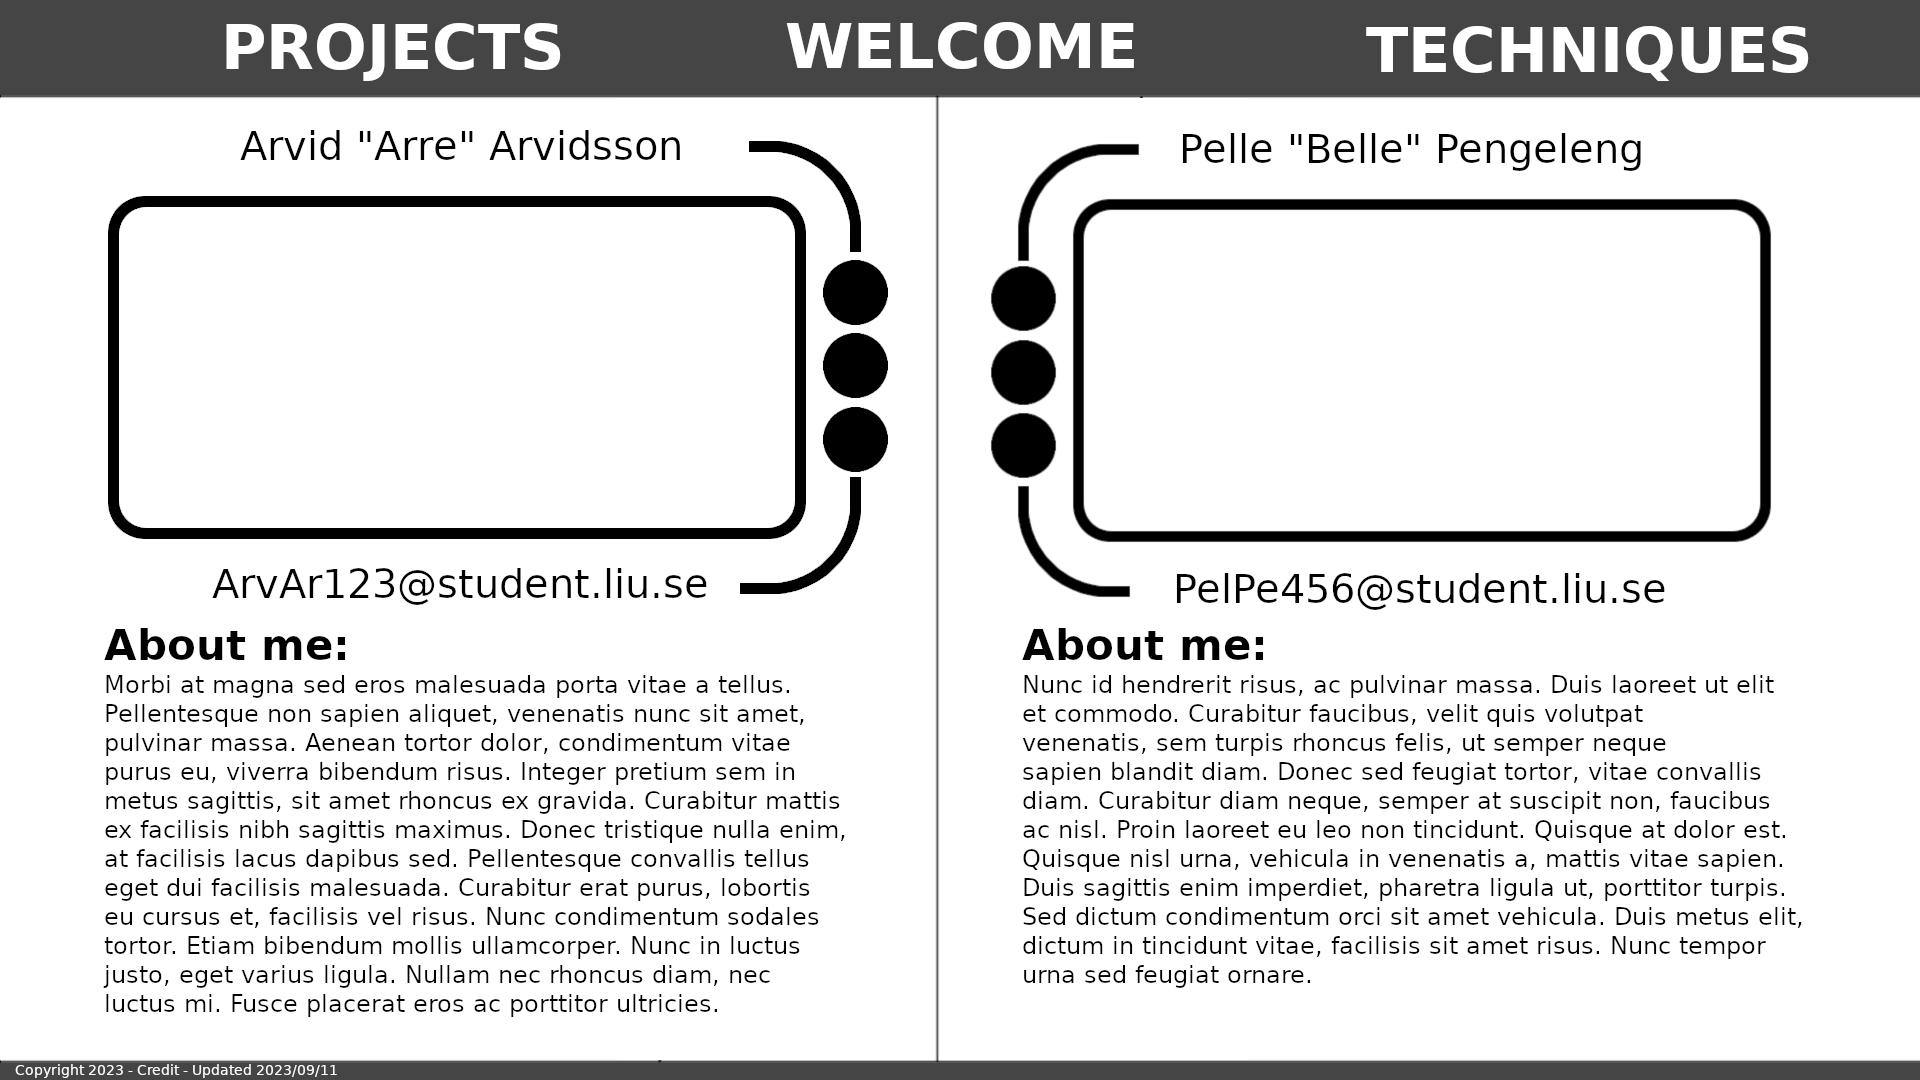
\includegraphics{LOFI Homepage}
    \caption{Startsida för presentationslagret; första-sidan nya besökare ser.}
    \label{fig:Low-Fidelity-Prototyp Homepage}
\end{figure}

    \subsubsection{Profilbild/ inforuta}
        Profilbilden består av en rektangel med en relevant bild inuti, ett fullständigt namn längst med översidan, en primär mejladdress längst med undersidan, och cirkulära genvägar längst med ena sidan. Genvägarna är personliga och kan ändras till vad personen använder. Namnet ska vara minst förnamn och efternamn men mellannamn och smeknamn är tillåtna om det får plats innanför bredden av bilden. Kanterna av inforutan har linjer som följer konturen av inforutan.

    \subsubsection{Självbiografi}
        Under inforutan finns det en stor textruta där personen ska skriva en självbiografi om vem dom är. Självbiografin måste inte fylla hela rutan. Startsidan är inte tänkt att skrolla mycket eller någonting alls och därför ska självbiografin hållas inom ramen av en halv sida. För ökad läsbarhet emot vissa bakgrunder kan textrutan ha en transparent bakgrund som kontrasterar profilens bakgrund.

\newpage
\subsection{Söksida för projekt}
    För att söka upp projekt använder man sig av en söksida som man kommer till genom knappen "PROJECTS" på de flesta sidor. Överst hittar man en sökruta för fritext med en filterknapp som visar eller döljer taggväljaren och en sorteringsknapp. Man kan välja en eller flera taggar tillsammans med fritext för att hitta ett specifikt projekt eller för att leta efter en kategori av projekt. Under taggväljaren visas sökresultat i en bred kolumn. Se figur 2 för illustration.

    \begin{figure}[h!]
        \centering
        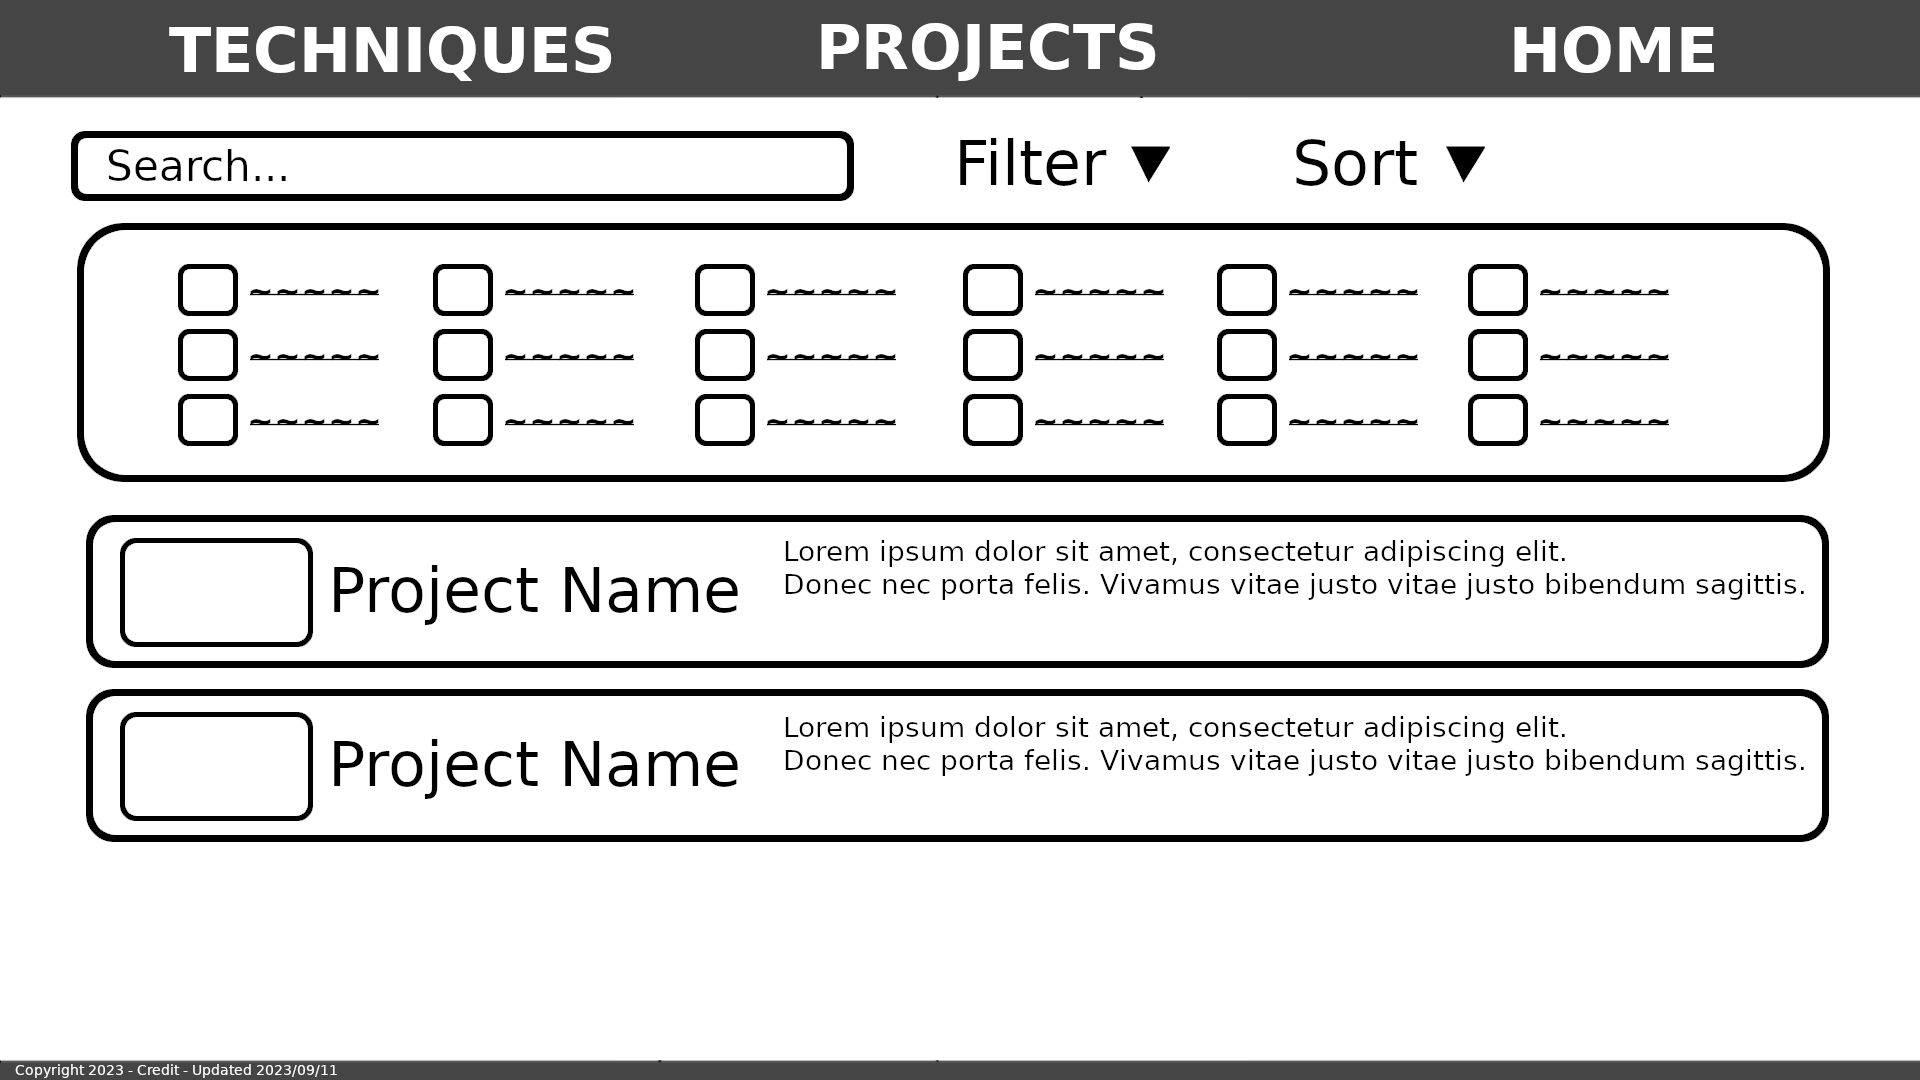
\includegraphics{LOFI Projects}
        \caption{Söksida för projekt. Tillåter användaren att leta efter projekt och ger en sammanfattning av projekten.}
        \label{fig:Low Fidelity-Prototyp Projects}
    \end{figure}

    \subsubsection{Sökfält}
        Längst upp finns ett sökfält som låter användaren söka efter ett projekt med fritext. Texten matchar projektnamnet och är inte skiftlägeskänslig. Höger om sökfältet finns en sorteringsknapp som ändrar hur sökresultaten skrivs ut. Användaren kan använda sorteringsknappen för att sortera resultaten i stigande eller fallande ordning och efter till exempel namn, start- \& slutdatum, eller kurs. Höger om den finns det en filterknapp som visar eller döljer en ruta under sökfältet där användaren kan välja en eller flera taggar för att filtrera sina sökresultat. Varje tagg står för en unik teknik som används i projekt. Höger om den, och längst till höger, finner användaren en knapp som visar en drop-down meny med val över fält att söka i när fritext används.

    \subsubsection{Sökresultat}
        Resterande utrymme på sidan används till sökresultaten. Varje sökresultat presenteras som en bred rektangel med en ikon eller bild till vänster, ett projektnamn i stor text bredvid ikonen, och en sammanfattning till höger. Sammanfattningen skall vara några meningar lång och ej längre än maximalt tre rader vid 100\% skala för att få plats i resultatrutan. Skulle texten råka överflöda storleken av resultatrutan (till exempel om webbläsaren skalas om) måste rutan skalas om för att få plats med sammanfattningen.

\newpage
\subsection{Söksida för metoder \& tekniker}
    På denna undersida hittar användaren en lista på alla olika tekniker som projekten använder. Det finns ingen sökmetod på denna sida utan alla tekniker är listade uppifrån ned. I rutan för varje teknik finns det en ikon/ symbol för tekniken, ett namn på tekniken, en mycket kort beskrivning på vad tekniken är, och en räknare för hur många projekt som använder den tekniken. Man kan klicka på antingen bilden eller namnet på tekniken för att komma till söksidan för projekt (se avsnitt 2.3: Söksida för projekt) med sökkriterierna ifyllda så att den filtrerar efter alla projekt som använder den tekniken. Se figur 3 för en illustration; notera exempelinnehållen i figuren.

    \begin{figure}[h!]
        \centering
        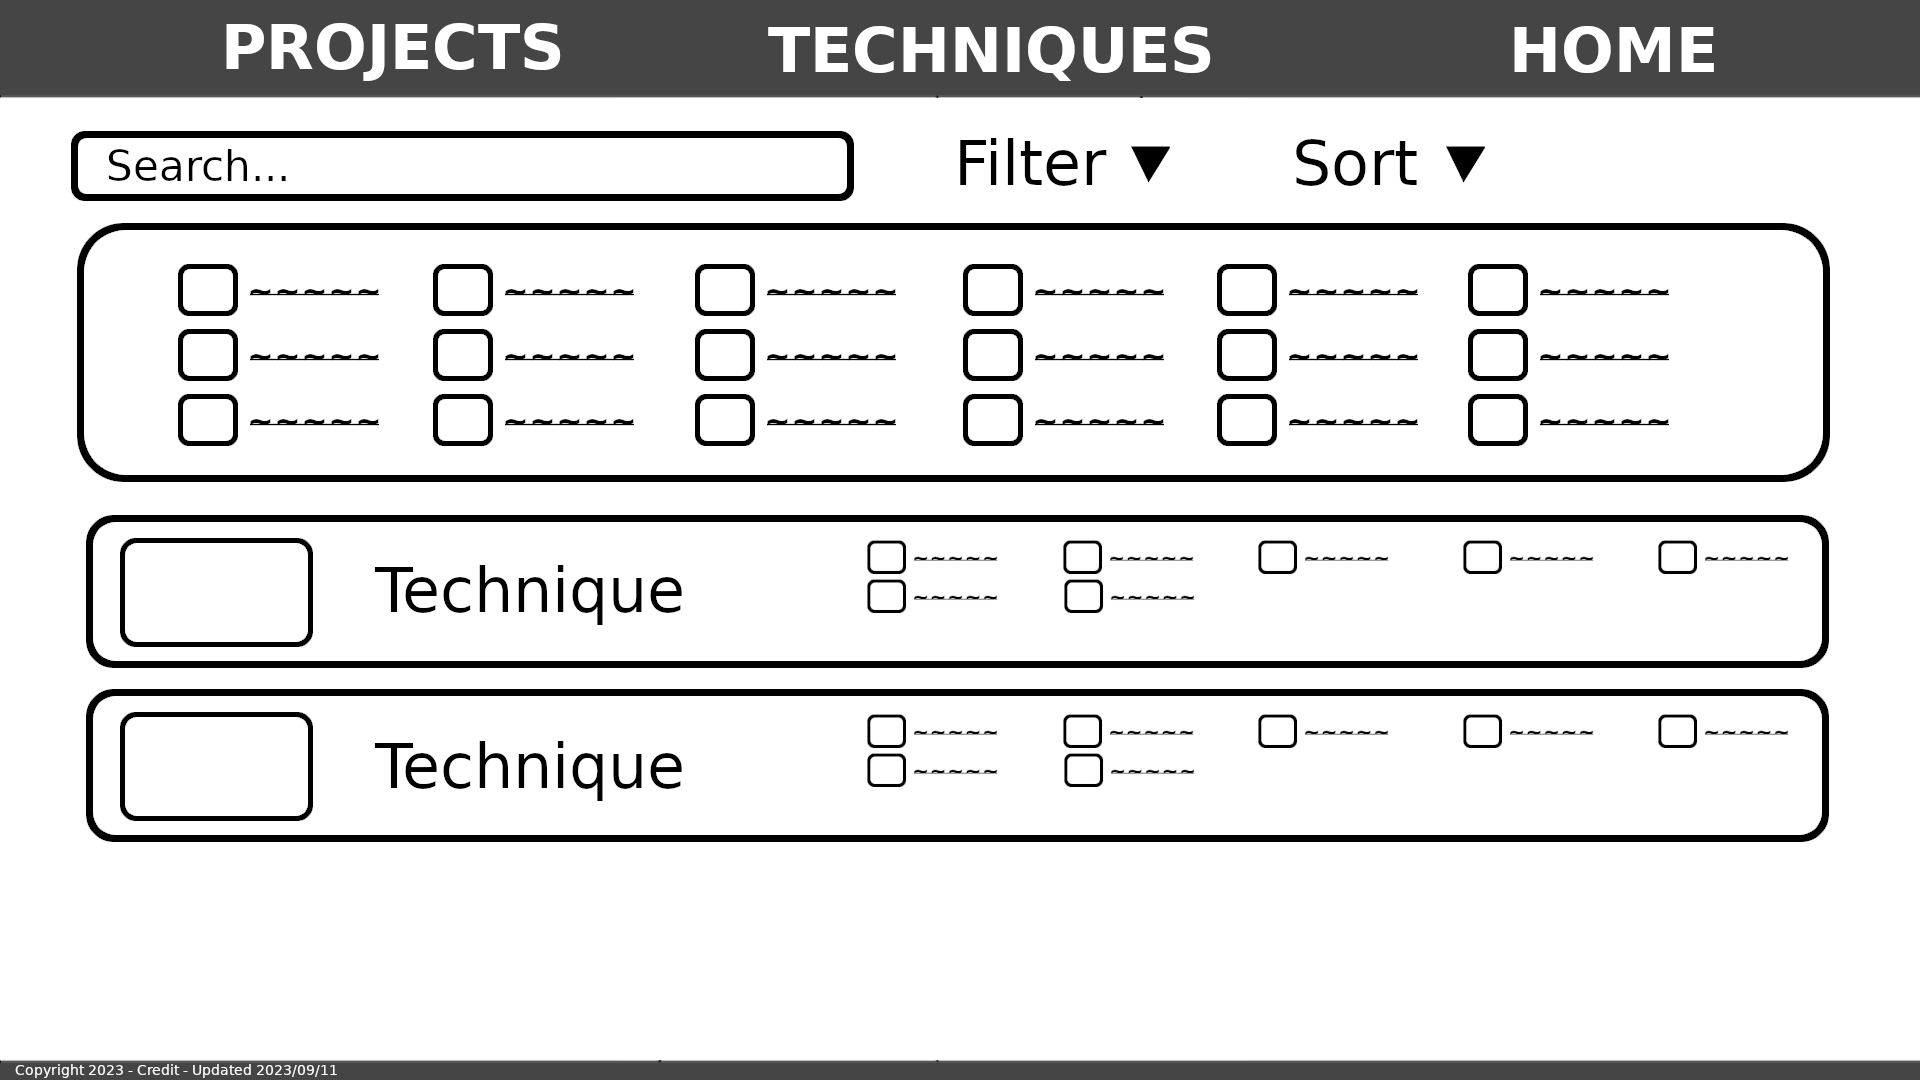
\includegraphics{LOFI Techniques}
        \caption{Söksida för metoder \& tekniker. Användare kan söka efter olika metoder som används i projekt.}
        \label{fig:Low-Fidelity-Prototyp Techniques}
    \end{figure}

\newpage
\subsection{Projektsida}
    Efter användaren klickar på ett sökresultat från söksidan (se avsnitt 2.3: Söksida för projekt) skickas användaren till projektsidan. Projektsidan visar en större bild på projektet och har djupgående dokumentation om projektet. Det finns också en faktaruta bredvid bilden som håller kort och konkret fakta om projektet. Se figur 4 för illustration. Notera att tabellen och 'Lorem Ipsum'-texten är exempelinehåll.

    \begin{figure}[h!]
        \centering
        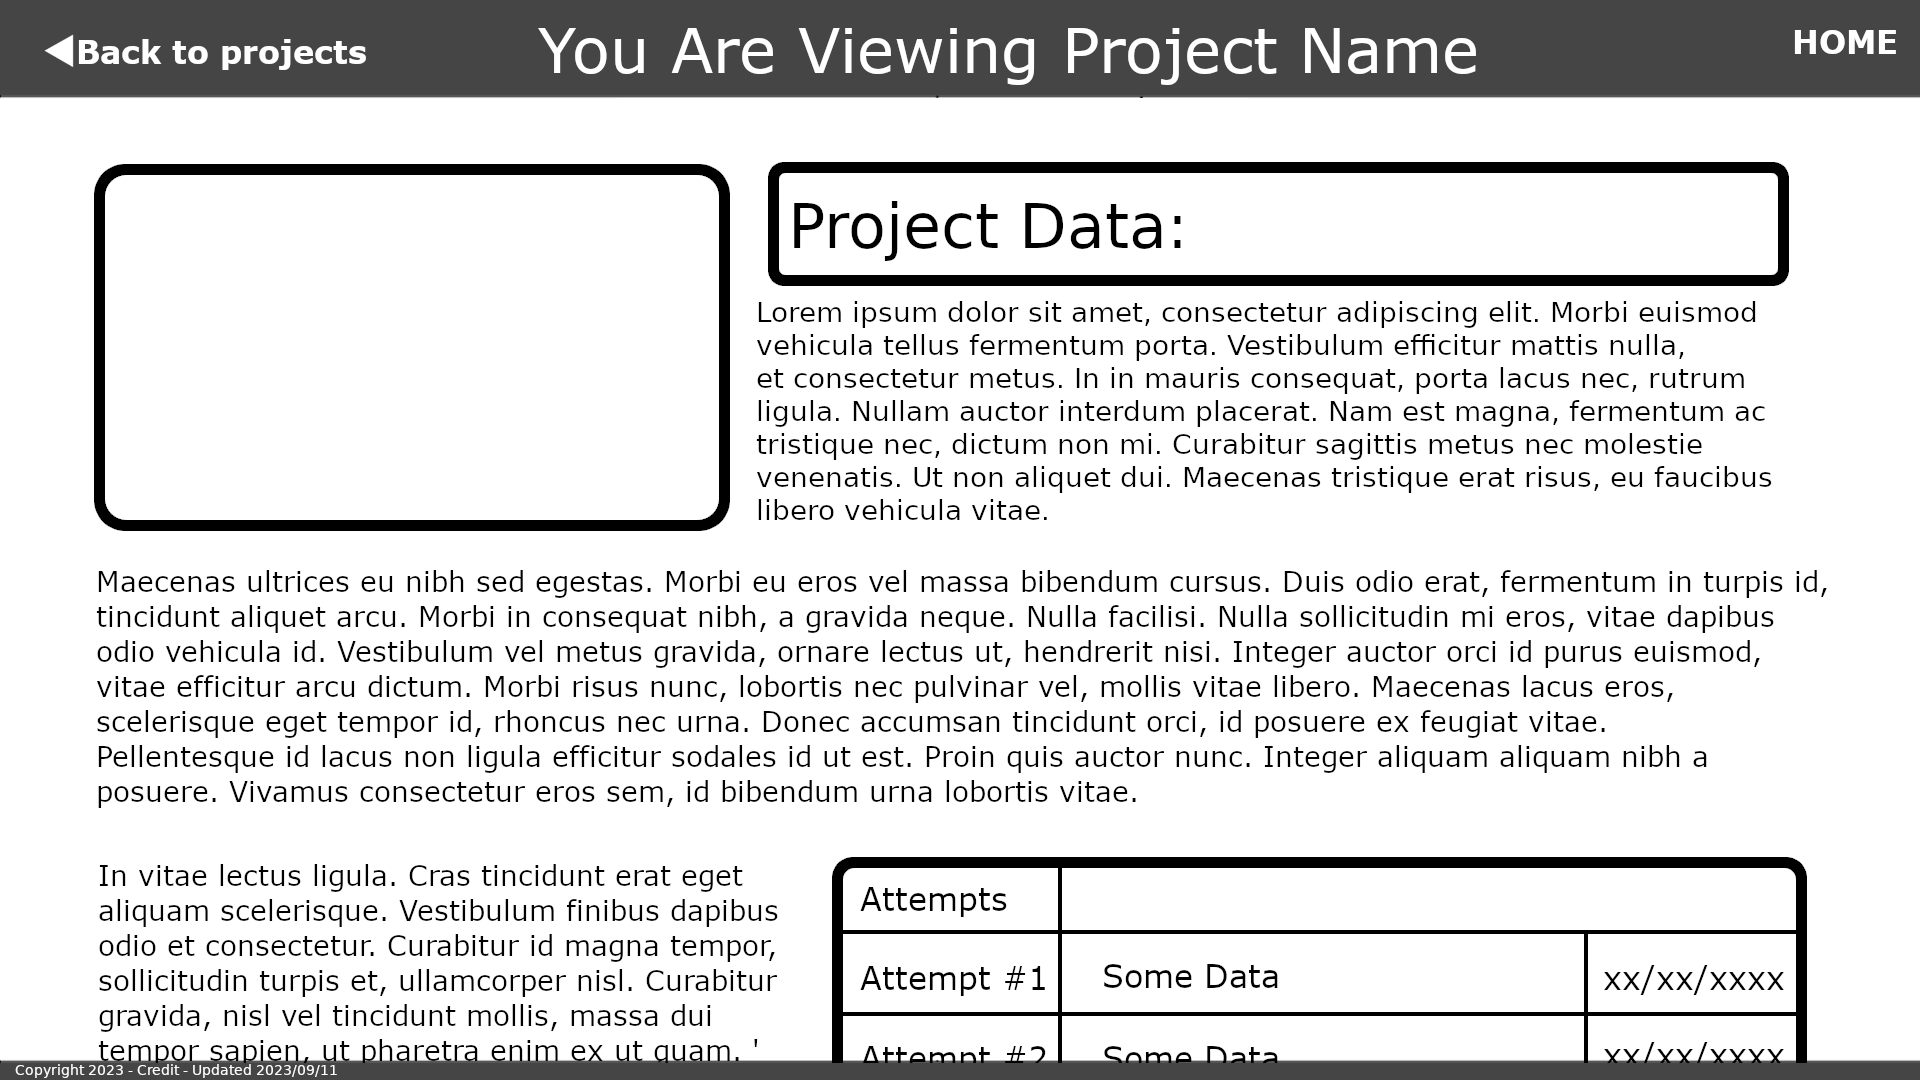
\includegraphics{LOFI Project Page}
        \caption{Layout för en projektsida med exempelinnehåll.}
        \label{fig:Low-Fidelity-Prototyp Project Page}
    \end{figure}

    \subsubsection{Bild, faktaruta, och text}
        Bilden är en förstorad bild av ikonen som finns för projektet från söksidan. Faktarutan (titlad "Project Data" i illustrationen) innehåller kort data om projektet som start- och slutdatum, projektnamn, kursnamn \& kurskod (om lämpligt), deltagare och/ eller ägare. Många fält i faktarutan är klickbara och tar användaren till en relevant destination, som till exempel kurshemsidan genom kurskoden. Under faktarutan och till höger om bilden finns det en längre sammanfattning av projektet. Därefter följer projektsidan ett traditionellt dokumentflöde med textstycken och bilder. Notera 'Lorem Ipsum'-texten samt tabellen i illustrationen vilket representerar ett exempel på hur innehållet av ett projekt kan se ut.

\end{document}
